% $Author: stef $
% $Date: 2008-04-04 17:14:31 +0200 (Fri, 04 Apr 2008) $
% $Revision: 318 $
%=================================================================
\ifx\wholebook\relax\else
% --------------------------------------------
% Lulu:
    \documentclass[a4paper,10pt,twoside]{book}
    \usepackage[
        papersize={6in,9in},
        hmargin={.75in,.75in},
        vmargin={.75in,1in},
        ignoreheadfoot
    ]{geometry}
    \input{../common.tex}
    \pagestyle{headings}
    \setboolean{lulu}{true}
% --------------------------------------------
% A4:
%   \documentclass[a4paper,11pt,twoside]{book}
%   \input{../common.tex}
%   \usepackage{a4wide}
% --------------------------------------------
    \graphicspath{{figures/} {../figures/}}
    \begin{document}
%   \renewcommand{\nnbb}[2]{} % Disable editorial comments
    \sloppy
\fi

\chapter{Combining Methods}\label{cha:combiningMethods}

%%%%%%%%%%%%%%%%%%%%%%%%%%%%%%%%%%%%%%%%%%%%%%%%%%%%%%%%%%%%%%%%%%%%%%%%
% \begin{figure}[h]
% 	\centerline{\includegraphics{}}
% 	\caption{Ready-to-use files for the Macintosh.  
% 	\label{fig:macfiles}}
% \end{figure}

% %%%%%%%%%%%%%%%%%%%%%%%%%%%%%%%%%%%%%%%%%%%%%%%%%%%%%%%%%%%%%%%%%%%%%%%%
% \begin{exofigwithsize}[0.5]{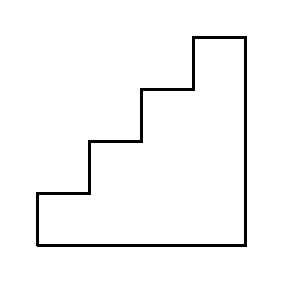
\includegraphics[width=3cm]{turtleMSmallStairs}}{A Staircase}\label{xp:letterA}
% You are not limited in your robot drawings to squares. You can create a wide range of geometrical figures.
% For example, here is a drawing of a small staircase. Write a script to reproduce this drawing. 
% \end{exofigwithsize}
% 
% \begin{exonofigtitle}{Moving Clock Hands}
% Experiment with different angle values for each of the two robots; that is,change the angle values for the two turn 
% methods. Then, compare the effect of the method \ct{turnLeft: 60} (for pica) and \ct{turnRight: 300} (for daly). 
% You can see that turning left 60 degrees yields the same result as turning right 300 degrees. This is so because 
% the sum of the two values is 360 degrees, that is, a full circle. 
% \end{exonofigtitle}
% 
% %%%%%%%%%%%%%%%%%%%%%%%%%%%%%%%%%%%%%%%%%%%%%%%%%%%%%%%%%%%%%%%%%%%%%%%%
% \begin{scriptfigwithsize}[0.4]{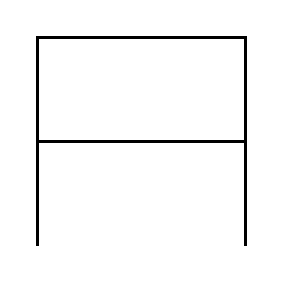
\includegraphics[width=5cm]{turtleMLetterA}}{The letter A}\label{scr:letterA}
% 	| pica | 
% 	pica := Bot new. 
% 	pica north. 
% 	pica go: 100. 
% 	pica east. 
% 	pica go: 100. 
% 	pica south. 
% 	pica go: 100. 
% 	pica north. 
% 	pica go: 50. 
% 	pica west. 
% 	pica go: 100
% \end{scriptfigwithsize}
% 
% \begin{script}[myster1]{What does pica do? (Problem 1)}
% 	| pica | 
% 	pica := Bot new. 
% 	pica go: 100. 
% 	pica turnLeft: 45. 
% 	pica go: 50. 
% 	pica turnLeft: 45. 
% 	pica go: 100 
% \end{script}


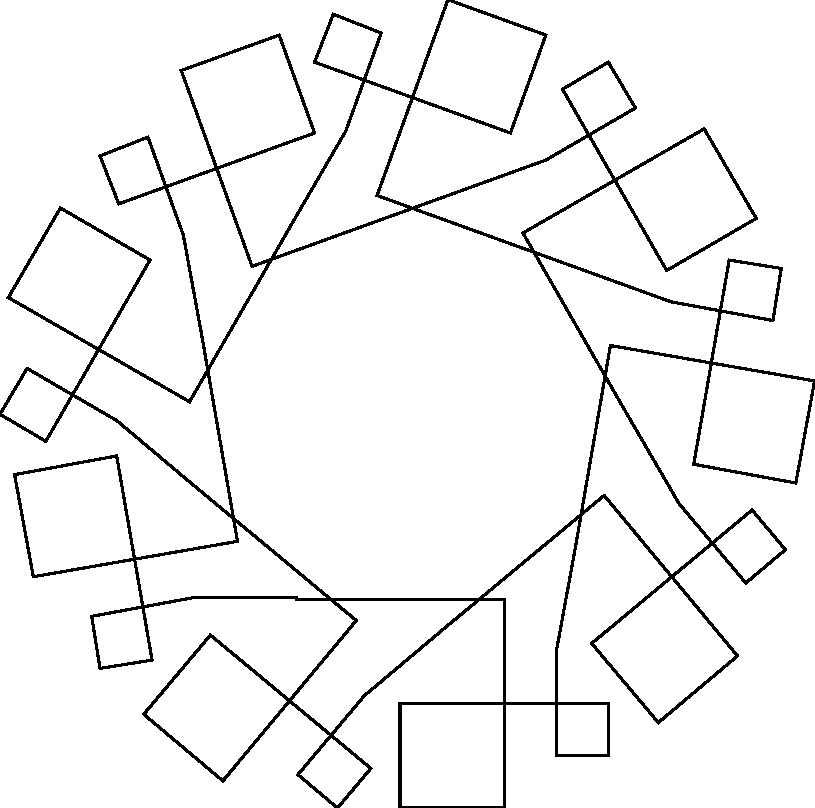
\includegraphics[width=0.45\linewidth]{compArtNouveauTurningScr}
\vspace*{1cm}

In Chapter~\ref{cha:methods}, you learned how to define methods. I showed that defining methods is interesting and useful because (1) methods save you from having to rewrite scripts, which is 
time-consuming and subject to error, and (2) methods can be used and reused by different 
robots. The other main advantage of using methods is the possibility of using methods in 
other methods, that is, calling one or more existing methods as part of the definition of a 
new method. The reuse of methods is what we will explore in this chapter. 

Being able to reuse methods is extremely important, because we can define a method 
in terms of another one without having to know all the details of how the second method is 
defined. We just call it and ask it to do what it is designed to do. 


\section{Nothing Really New: The Square Method Revisited} 

Having methods call other methods (which we call composing methods) is quite natural and 
is not really new. In fact, it is what you did in Chapter~\ref{cha:methods} when you defined a method! The 
method \ct{square} includes in its definition calls to the methods \ct{turnLeft:}, \ct{go:}, and \ct{timesRepeat:} 
(as shown in Method~\ref{mth:131}). Thus even the simple method squareis defined in terms of other 
methods, and we did not have to know how \ct{turnLeft:}, \ct{go:}, and \ct{timesRepeat:} are defined. We 
needed to know only what they do. So we are essentially done with this chapter, with nothing 
left to do but have some fun. 


\begin{method}[131]{}
!\textbf{square}!
"Draw a square of 100 pixels wide " 
4 timesRepeat: 
[ self go: 100; 
turnLeft: 90 ] 
\end{method}

\section{Other Graphical Patterns} 

In Chapter~\ref{cha:methods}, I asked you to define the method pattern, which draws a simple abstract pattern (See script~\ref{scr:125}). Now I will ask you to perform some further experiments that will 
produce more drawings by defining more methods. 

\begin{exofigwithsize}[0.5]{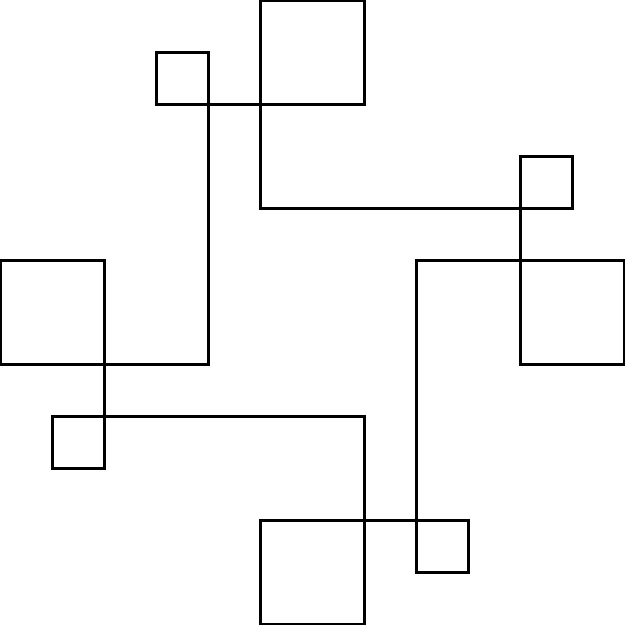
\includegraphics[width=5cm]{compCompleteThing}}{}\label{xp:131}
Define a method \ct{pattern4} that calls \ct{pattern} four times to produce the figure below. You will use this method 
later, in another script. After you have created the method \ct{pattern4}, use the following three-line script to make 
pica draw the figure.


\ct{| pica |} \\
\ct{pica := Bot new.} \\
\ct{pica pattern4 }

\end{exofigwithsize}


\begin{exonofigtitle}{A Ferris Wheel}
Define a method called \ct{tiltedPattern} that draws the picture at the beginning of this chapter, which looks 
somewhat like a Ferris wheel. Hint: you will have to call \ct{pattern} nine times, and the angle through which to turn 
between calls is 10 degrees. 
\end{exonofigtitle}


\begin{exofigwithsize}[0.5]{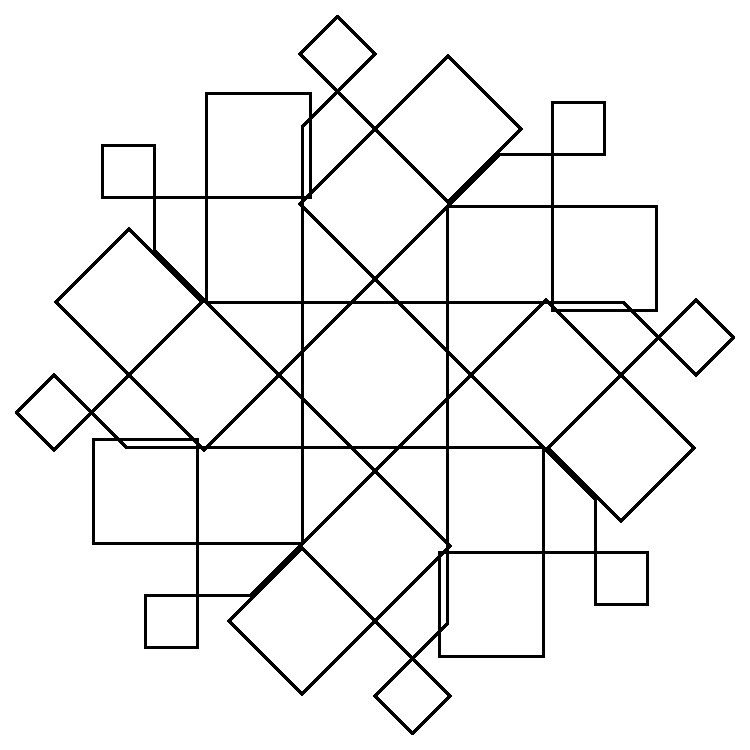
\includegraphics[width=5cm]{compArtNouveauGiantScr}}{Doubling the Frame}\label{xp:133}
Define the method \ct{doubleFrame}, presented below,that draws the picture shown after the method definition. 


\textbf{doubleFrame}\\
\ct{8 timesRepeat:} \\
\ct{[ self pattern.} \\
\ct{self turnLeft: 45.} \\
\ct{self go: 100 ]} 
\end{exofigwithsize}


\section{What Do These Experiments Tell You?} 

Now let’s see what you can learn from the experiments you did. As you can see from the methods \ct{pattern4}, \ct{tiltedPattern}, and \ct{doubleFrame}, the method \ct{pattern} was defined only once, 
and then \emph{reused several times} in different methods. Defining patternas a method allows you 
to (1) define it only once, (2) reuse it in various contexts, and (3) not introduce errors by copying this method over and over. 

If you look at the definition of the method doubleFrame, you see that it is defined in terms 
of the \ct{pattern} method, which is itself defined in terms of other methods, such as \ct{go:} and 
\ct{turnLeft:}. In fact, a complex method is often defined in terms of simpler methods, which 
themselves are defined in terms of even simpler methods, which themselves are defined in 
terms of even simpler methods, which themselves\ldots. The advantage of this is that it is easier 
to understand and to define simple methods than complex methods, and the technique of 
defining methods in terms of simpler methods limits the degree of complexity in any one 
method. In Chapter~\ref{cha:decomposing}, I will show you that to solve a problem, it is advantageous to decompose it into smaller subproblems, solve these subproblems, and then use the solutions to the smaller subproblems to solve the main problem. 


It is essential to understand that in defining the method \ct{doubleFrame}, you do not have to 
know how \ct{pattern} is defined. You just need to know what it does and how to use it! When we 
define a method, we are giving a single name to a sequence of messages, which reduces the 
number of details that we have to keep track of. We just have to remember what the method 
does and its name, not how it does it. We say that we are building an \emph{abstraction} over the definition details. 

To make this point clear, I rewrote the method \ct{doubleFrame} without calling the method 
patternby directly copying the definition of pattern(shown in italics). Compare \ct{doubleFrame} 
\ct{WithoutCallingPattern} (Method~\ref{mth:132}) with the method \ct{doubleFrame}. The new version without 
\ct{pattern} is not only longer, but for most people it is also more confusing and harder to understand. 

Now imagine what would happen if I did the same with the code of \ct{turnRight:}, \ct{turnLeft:}, 
and \ct{go:} --- because these are methods too. It would be a nightmare! There would be so many 
details that we would be lost all the time.


\begin{method}[132]{Creating the double frame without the abstraction of the pattern method}
!\textbf{doubleFrameWithoutCallingPattern}!

8 timesRepeat: 
[ self go: 100. 
self turnRight: 90. 
self go: 100. 
self turnRight: 90. 
self go: 50. 
self turnRight: 90. 
self go: 50. 
self turnRight: 90. 
self go: 100. 
self turnRight: 90. 
self go: 25. 
self turnRight: 90. 
self go: 25. 
self turnRight: 90. 
self go: 50. 
self turnLeft: 45. 
self go: 100 ]
\end{method}


\important{When you write a new method,it can call other methods.You can use a method without 
knowing how it is written.After you finish writing a method,you can call it when you write another method.}


\section{Squares Everywhere} 

Now it is time to practice. Define the following methods using the method square. 

\begin{exonofigtitle}{Some Boxes}
Define methods boxandseparatedBoxthat produce the pictures shown in Figure~\ref{fig:131}. 
\end{exonofigtitle}


\begin{figure}[h]
	\centerline{\hfill\includegraphics[width=0.45\linewidth]{comp4Squares}\hfill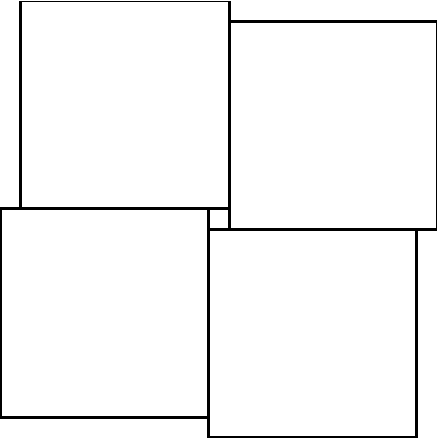
\includegraphics[width=0.45\linewidth]{comp4SquaresTwo}\hfill}
	\caption{Boxes
	\label{fig:131}}
\end{figure}


\begin{exonofigtitle}{Your Choice}
Use your previous methods to generate various figures of your choice.Have fun! 
\end{exonofigtitle}


\begin{exonofigtitle}{A Star}
Using the method \ct{box}, experiment and define a method \ct{star} that produces the right-hand picture in Figure~\ref{fig:132}.
\end{exonofigtitle}

\begin{figure}[h]
	\centerline{\hfill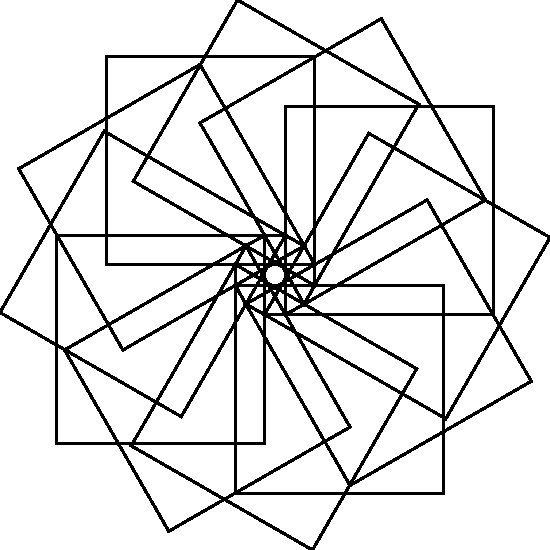
\includegraphics[width=0.45\linewidth]{comp4SquaresThree}\hfill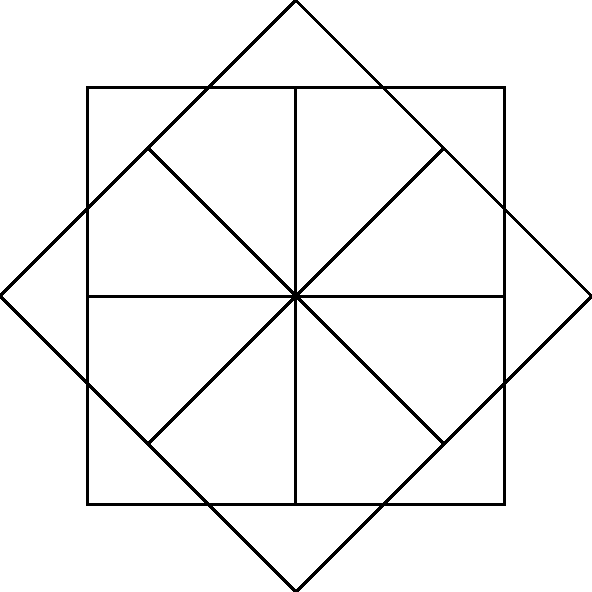
\includegraphics[width=0.45\linewidth]{comp4SquaresFour}\hfill}
	\caption{Stars
	\label{fig:132}}
\end{figure}

\section{Summary} 

\begin{itemize}
	\item When you write a new method, it can call other methods. 
	\item You can use a method without knowing how it is written; you need to know only what does. 
	\item After you finish writing a method, you can call it when you write other methods. 
	\item Hiding the details of a method by giving it a name is called \emph{abstraction}. 
\end{itemize}

\ifx\wholebook\relax\else
    \end{document}
\fi

%%% Local Variables:
%%% coding: utf-8
%%% mode: latex
%%% TeX-master: t
%%% TeX-PDF-mode: t
%%% ispell-local-dictionary: "english"
%%% End:
